% By Sai Avula
% Edited by Audrey Beard
\documentclass[11pt]{article}
\usepackage[utf8]{inputenc}
\usepackage{listings}
\usepackage{upquote,textcomp}
\usepackage{amsmath,amsfonts,amsthm}
\usepackage{url}
\usepackage{graphicx}
\usepackage{fullpage}
\usepackage{hyperref}

\usepackage{color}

% Hard figure placement
\usepackage{float}

\usepackage[coloroftodonotes]{todonotes}

\definecolor{mygreen}{rgb}{0,0.6,0}
\definecolor{mygray}{rgb}{0.5,0.5,0.5}
\definecolor{mymauve}{rgb}{0.58,0,0.82}

\newcommand{\audrey}[1]{\todo[color=pink]{#1}}


\lstset{frame=tb,
  language=,
  aboveskip=3mm,
  belowskip=3mm,
  showstringspaces=false,
  columns=flexible,
  keepspaces=true,
  basicstyle={\small\ttfamily},
  numbers=none,
  numberstyle=\tiny\color{black},
  keywordstyle=\color{black},
  commentstyle=\color{black},
  stringstyle=\color{black},
  breaklines=true,
  breakatwhitespace=true,
  tabsize=3
}

\lstset{frame=tb,
  language=Python,
  aboveskip=3mm,
  belowskip=3mm,
  showstringspaces=false,
  columns=flexible,
  basicstyle={\small\ttfamily},
  numbers=none,
  numberstyle=\tiny\color{mygray},
  keywordstyle=\color{blue},
  commentstyle=\color{mygreen},
  stringstyle=\color{mymauve},
  breaklines=true,
  breakatwhitespace=true,
  tabsize=3
}

\textwidth  6.5in
\oddsidemargin +0.0in
\evensidemargin +0.0in
\textheight 9.0in
\topmargin -0.5in

\setlength{\parindent}{0pt}
\setlength{\parskip}{3pt}


\setcounter{part}{1}

\newenvironment{Part}[2]
{
    \begin{center}
        \Large\textbf{Part \thepart: #1}\\
        \large\textit{#2}
        \stepcounter{part}
    \end{center}
}

\newcommand{\duedate}[1]{\date{\textbf{Due: #1}}}


\title{\textbf{Build Your Own Choose-Your-Own-Adventure Game}}
\author{\textit{Custom Class Structures, Loops, Node and Tree Diagrams, Game Design and Development}}
\duedate{\todo{Due date}}


\begin{document}
\thispagestyle{empty}

\maketitle
\begin{Part}{Designing Your Story}{Write and create structural framework of the story}

In this part you will be writing your own choose-your-own adventure story which should focus on or be based around one or more of the topics that were explored in the readings for the previous assignments. There is no limit to how creative the story can be, but it should have a clear structure and progression of events. After developing the story, you will create a visual representation of your story in the form of a \textbf{Storyboard}, which will contain nodes such as \textbf{Storypoints}, as seen in the diagram below.


A \textbf{divergence} is a branching point in the story where the player can make two or more choices that lead to different events.

A \textbf{convergence} is a story event that can be reached by more than one path.

\textbf{Path length} is the number of “steps” needed to get from the starting event to a specified ending event. In Figure \ref{fig:graph-terminology}, for example, every path in the graph has a path length of four.

An \textbf{ending event} is a point that concludes the story, and gives the players the option to end the story or restart the game.

Each Storypoint will function as a point in the story where the user can make a decision to progress further in the game, as it either must terminate or branch out to at least 2 other child Storypoint\audrey{define} nodes. In order to build a rich story and demonstrate your comprehension, your graph should have:
\begin{itemize}
    \item A minimum path length of 3
    \item At least one path of length 4
    \item No more than 3 children for any single node
    \item At least 4 divergences
    \item At least 1 convergence
    \item At least 3 possible endings
\end{itemize}


\audrey{what's this section doing here?}


\begin{figure}[H]
    \centering
    \fbox{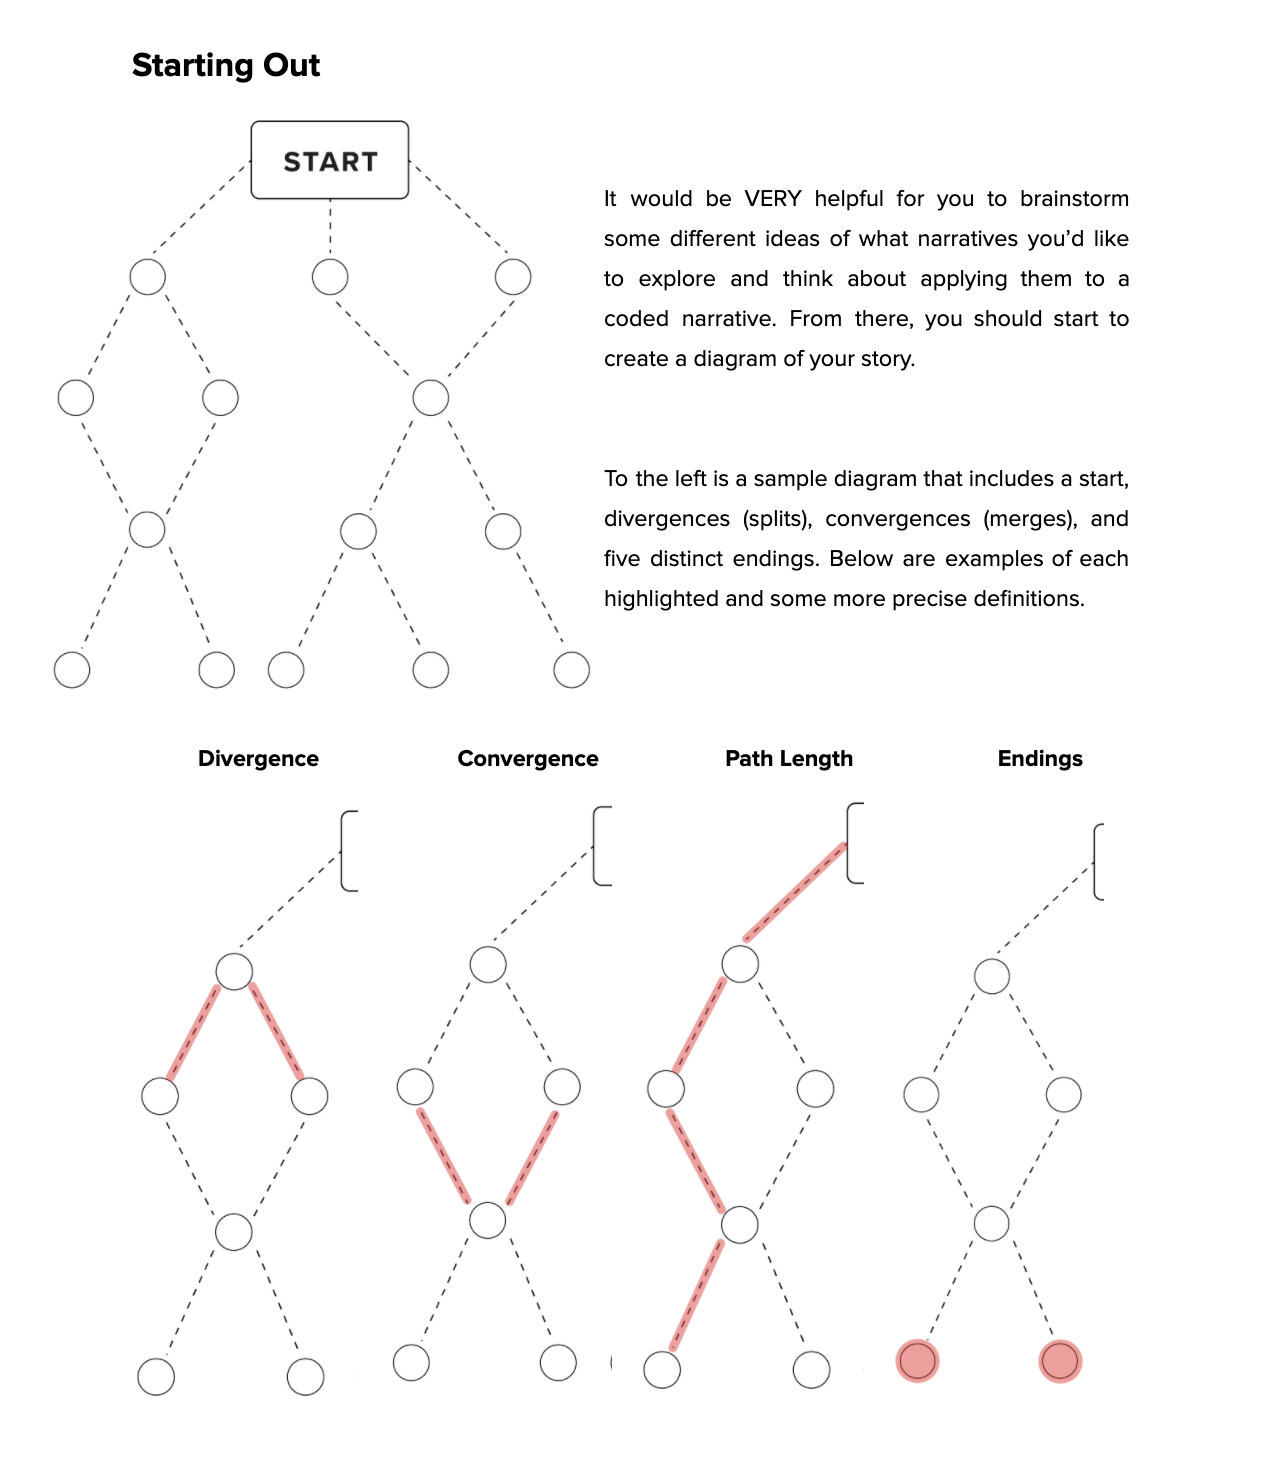
\includegraphics[width=0.9\textwidth]{Homework/HW8_Games-Adventure-Story/images/graph-terminology.png}}
    \caption{Examples of various graph sub-structures}
    \label{fig:graph-terminology}
\end{figure}

\end{Part}

\begin{Part}{Building Your Custom Classes}{Creating the Storypoint, Storyboard, and Driver Classes}
Next, you will be implementing the function of the game through three custom classes:

\begin{itemize}
    \item Storypoint - this class should act as a template for the nodes mentioned above. It should contain a list of children (subsequent events in the game progression), the text to be displayed at the corresponding point in the game, and a list of the user-input commands that will be used to continue to the next Storypoint.
    
    \item Storyboard - the purpose of this class is to contain the initial Storypoint (beginning node), ending Storypoints, and rest of the Storypoints, as well as contain any additional helper functions.
    
    \item Driver - this class will be used to navigate the Storyboard. It will be used to keep track of the current Storypoint, any previous Storypoints, and any data or statistics that are pertinent to decisions in the game (character information etc.)
    

\end{itemize}
\end{Part}

\begin{Part}{Implementing the Classes}{Putting it All Together}
In this part, you will use the classes you created in the previous section to create the choose-your-own-adventure game. As stated previously, each decision in the story must have its own Storypoint and options of user input that will allow the user to move to the next point in the story. The game should also allow the user to “play” as many times as they want (until they enter a specific end command). It should also output all the decisions the user had made in the play-through as well as any other relevant data after the user ends the game. Make sure to thoroughly test all possible paths to ensure there is a continuous and coherent flow to the game, especially in cases of user error. Also make sure it adheres to the structural requirements above. All paths should lead to an ending event.
\end{Part}

\begin{Part}{README}{Final Thoughts}
Please respond to the questions in the provided README.txt file and submit it along with your code.
\end{Part}

\end{document}
